\documentclass{article}
\usepackage{parskip}
\usepackage{caption}
\usepackage{subcaption}
\usepackage{multirow}
\usepackage{float}
\usepackage{booktabs}
%\usepackage[annataritalic]{tengwarscript}

% Language setting
% Replace 'english' with e.g. 'spanish' to change the document language
\usepackage[italian]{babel}
\addto\captionsenglish{\renewcommand{\figurename}{Figura}}

% Set page size and margins
% Replace 'letterpaper' with 'a4paper' for UK/EU standard size
\usepackage[letterpaper,top=2cm,bottom=2cm,left=2cm,right=2cm,marginparwidth=1.75cm]{geometry}

% Useful packages
\usepackage{amsmath}
\usepackage{graphicx}
\graphicspath{ {./images/} }
\usepackage[colorlinks=true, allcolors=blue]{hyperref}


\usepackage{listings}
\usepackage{xcolor}

\definecolor{codegreen}{rgb}{0,0.6,0}
\definecolor{codegray}{rgb}{0.5,0.5,0.5}
\definecolor{codepurple}{rgb}{0.58,0,0.82}
\definecolor{backcolour}{rgb}{0.95,0.95,0.92}

\lstdefinestyle{mystyle}{
    backgroundcolor=\color{backcolour},   
    commentstyle=\color{codegreen},
    keywordstyle=\color{magenta},
    numberstyle=\tiny\color{codegray},
    stringstyle=\color{codepurple},
    basicstyle=\ttfamily\footnotesize,
    breakatwhitespace=false,         
    breaklines=true,                 
    captionpos=b,                    
    keepspaces=true,                 
    numbers=left,                    
    numbersep=5pt,                  
    showspaces=false,                
    showstringspaces=false,
    showtabs=false,                  
    tabsize=2
}

\lstset{style=mystyle, language= C++}

\begin{document}
\begin{center}
    {\Large Alma Mater Studiorum - Università di Bologna}
    
    \vspace{0.5cm}
    {\bf \large Relazione per il corso di Data Science}
\end{center} 

\noindent
{Liam Cavini} \hfill {\bf 6° Foglio, Dati ad alta dimensione}\\
{\ Semestre Invernale 2024/2025} \hfill 24/11/2024

\subsection*{Risorse}
Il codice utilizzato, insieme al file .tex di questo documento, possono essere trovati nella seguente repository github: \url{https://github.com/LazyLagrangian/data_science}.

\subsection*{Esercizio 1 - Auto-facce e algoritmo PCA }
Per lo svolgimento dell'esercizio è stato fornito un dataset di immagini di volti, ciascun immagine su una scala di grigi (quindi ogni pixel è identificato con un singolo numero) di dimensione $168 \times 192$ pixel.
Ciascuna immagine può dunque essere vista come un datapoint di dimensione $d = 32256$.

Sul dataset è stata svolta l'analisi delle componenti principali (PCA), trovando le autofacce (autovettori nello spazio di dimensione $d$ di queste immagini).
Le prime autofacce del dataset (a cui è stata sottratta la faccia media), sono mostrate in figura \ref{fig:eigenfaces}.
\begin{figure}[H]
    \centering
    \begin{subfigure}[b]{0.29\textwidth}
        \centering
        \includegraphics[width=\textwidth]{immagini/eigenface_0.png}
    \end{subfigure}
    \begin{subfigure}[b]{0.29\textwidth}
        \centering
        \includegraphics[width=\textwidth]{immagini/eigenface_1.png}
    \end{subfigure}
    \begin{subfigure}[b]{0.29\textwidth}
        \centering
        \includegraphics[width=\textwidth]{immagini/eigenface_2.png}
    \end{subfigure}
    \begin{subfigure}[b]{0.29\textwidth}
        \centering
        \includegraphics[width=\textwidth]{immagini/eigenface_3.png}
    \end{subfigure}
    \begin{subfigure}[b]{0.29\textwidth}
        \centering
        \includegraphics[width=\textwidth]{immagini/eigenface_4.png}
    \end{subfigure}
    \begin{subfigure}[b]{0.29\textwidth}
        \centering
        \includegraphics[width=\textwidth]{immagini/eigenface_5.png}
    \end{subfigure}
    \begin{subfigure}[b]{0.29\textwidth}
        \centering
        \includegraphics[width=\textwidth]{immagini/eigenface_6.png}
    \end{subfigure}
    \begin{subfigure}[b]{0.29\textwidth}
        \centering
        \includegraphics[width=\textwidth]{immagini/eigenface_7.png}
    \end{subfigure}
    \begin{subfigure}[b]{0.29\textwidth}
        \centering
        \includegraphics[width=\textwidth]{immagini/eigenface_8.png}
    \end{subfigure}
    \caption{\emph{Le prime nove autofacce del dataset modificato per avere media nulla.}}
    \label{fig:eigenfaces}
\end{figure}

I primi autovettori forniscono la direzione di maggior variazione del dataset. Dunque, se si scompone un immagine di un volto nella base delle autofacce, la proiezione sulle prime autofacce contiene più informazione sull'immagine che quelle sulle restanti componenti.
Se l'immagine non è un volto non ci aspettiamo che questo sia il caso. Per valutare questa ipotesi si è compiuta la scomposizione in autofacce di tre immagine non appartenenti al dataset, una di un volto, una di un cane e una di una pianta.

Le tre immagine originali sono mostrate in figura \ref{fig:immagini_originali}.

\begin{figure}[H]
    \centering
    \begin{subfigure}[b]{0.29\textwidth}
        \centering
        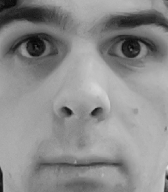
\includegraphics[width=\textwidth]{../liam_face2.png}
    \end{subfigure}
    \begin{subfigure}[b]{0.29\textwidth}
        \centering
        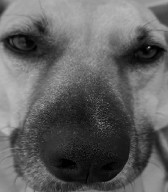
\includegraphics[width=\textwidth]{../lady_face.png}
    \end{subfigure}
    \begin{subfigure}[b]{0.29\textwidth}
        \centering
        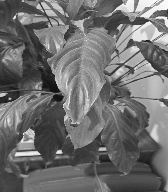
\includegraphics[width=\textwidth]{../plant.png}
    \end{subfigure}
    \caption{\emph{Le tre immagini originali.}}
    \label{fig:immagini_originali}
\end{figure}

La scomposizione in autofacce della immagine del volto è mostrata in figura \ref{fig:immagine_proiettata}.
\begin{figure}[H]
    \centering
    \begin{subfigure}[b]{0.29\textwidth}
        \centering
        \includegraphics[width=\textwidth]{immagini/liam_faccia_25.png}
    \end{subfigure}
    \begin{subfigure}[b]{0.29\textwidth}
        \centering
        \includegraphics[width=\textwidth]{immagini/liam_faccia_100.png}
    \end{subfigure}
    \begin{subfigure}[b]{0.29\textwidth}
        \centering
        \includegraphics[width=\textwidth]{immagini/liam_faccia_150.png}
    \end{subfigure}
    \begin{subfigure}[b]{0.29\textwidth}
        \centering
        \includegraphics[width=\textwidth]{immagini/liam_faccia_300.png}
    \end{subfigure}
    \begin{subfigure}[b]{0.29\textwidth}
        \centering
        \includegraphics[width=\textwidth]{immagini/liam_faccia_500.png}
    \end{subfigure}
    \begin{subfigure}[b]{0.29\textwidth}
        \centering
        \includegraphics[width=\textwidth]{immagini/liam_faccia_700.png}
    \end{subfigure}
    \begin{subfigure}[b]{0.29\textwidth}
        \centering
        \includegraphics[width=\textwidth]{immagini/liam_faccia_1000.png}
    \end{subfigure}
    \begin{subfigure}[b]{0.29\textwidth}
        \centering
        \includegraphics[width=\textwidth]{immagini/liam_faccia_2000.png}
    \end{subfigure}
    \begin{subfigure}[b]{0.29\textwidth}
        \centering
        \includegraphics[width=\textwidth]{immagini/liam_faccia_3000.png}
    \end{subfigure}
    \caption{\emph{Proiezione sui primi $r$ assi principali della immagine del volto.}}
    \label{fig:immagine_proiettata}
\end{figure}

Si è valutata quanta informazione contiene ogni autovalore per ciascuna delle tre immagini usando due metodi:
il primo consiste nel calcolare la somma dell'errore quadratico medio tra i pixel dell'immagine originale e della proiezione,
il secondo nel valutare il `structural similarity index' sempre tra questi due \footnote{\url{https://scikit-image.org/docs/stable/auto_examples/transform/plot_ssim.html}}.
I risultati ottenuti sono mostrati in figura \ref{fig:information_loss}.

\begin{figure}[H]
    \centering
    \begin{subfigure}[b]{0.49\textwidth}
        \centering
        \includegraphics[width=\textwidth]{immagini/msqe.png}
    \end{subfigure}
    \begin{subfigure}[b]{0.49\textwidth}
        \centering
        \includegraphics[width=\textwidth]{immagini/ssi.png}
    \end{subfigure}
    \caption{\emph{La figura è composta da due grafici, il primo partendo da sinistra mostra l'errore quadratico medio tra l'immagine originale e l'immagine ricostruita dai primi $r$ autovalori, mentre il secondo mostra il structural similarity index tra queste.}}
    \label{fig:information_loss}
\end{figure}

Come era atteso l'informazione sulla immagine della pianta contenuta nella proiezione sulle prime autofacce risulta minore rispetto al corrispondente per il volto. 

\subsection*{Esercizio 2 - Metodi PCA e t-SNE per la banca dati MNIST}
L'esercizio consiste nell'applicare i metodi PCA e t-SNE al dataset MNIST utilizzato nel precedente laboratorio.

In figura \ref{fig:confronto_numeri} sono mostrati alcuni elementi del dataset ricostruiti dalle prime $10$ componenti principali, comparati agli originali.
Queste dieci componenti contribuiscono rispettivamente il 9.7\%, 7.1\%, 6.1\%, 5.4\%, 4.9\%, 4.3\%, 3.3\%, 2.9\%, 2.8\% , 2.3\% della varianza totale, e quindi complessivamente il 48.9\%.

\begin{figure}[H]
    \centering
    \begin{subfigure}[b]{0.29\textwidth}
        \centering
        \includegraphics[width=\textwidth]{immagini/number_sample1.png}
    \end{subfigure}
    \begin{subfigure}[b]{0.29\textwidth}
        \centering
        \includegraphics[width=\textwidth]{immagini/number_sample2.png}
    \end{subfigure}
    \begin{subfigure}[b]{0.29\textwidth}
        \centering
        \includegraphics[width=\textwidth]{immagini/number_sample4.png}
    \end{subfigure}
    \begin{subfigure}[b]{0.29\textwidth}
        \centering
        \includegraphics[width=\textwidth]{immagini/number_rebuilt1.png}
    \end{subfigure}
    \begin{subfigure}[b]{0.29\textwidth}
        \centering
        \includegraphics[width=\textwidth]{immagini/number_rebuilt2.png}
    \end{subfigure}
    \begin{subfigure}[b]{0.29\textwidth}
        \centering
        \includegraphics[width=\textwidth]{immagini/number_rebuilt4.png}
    \end{subfigure}
    \caption{\emph{campioni del dataset messi a confronto con la loro ricostruzione ottenuta dagli autovalori associati alle prime dieci componenti principali.}}
    \label{fig:confronto_numeri}
\end{figure}

In figura \ref{fig:pca_numbers} sono mostrati i dati proiettati sulle prime due componenti principali.
Si osserva che non sarebbe possibile distinguere le categorie se non fossero colorate in modo diverso.

\begin{figure}[H]
    \centering
    \begin{subfigure}[b]{0.8\textwidth}
        \centering
        \includegraphics[width=\textwidth]{immagini/pca_numbers.png}
    \end{subfigure}
    \caption{\emph{La figura mostra la riduzione in due dimensioni del dataset MNIST, ottenuta attraverso il metodo PCA.}}
    \label{fig:pca_numbers}
\end{figure}

In figura \ref{fig:tnse_numbers} è mostrato il risultato della riduzione a due dimensioni ottenuta tramite il metodo t-SNE, applicata sull'intero dataset, e sul dataset ridotto alle prime $40$ componenti principali. Si nota che le categorie sono ben distinguibili.
\begin{figure}[H]
    \centering
    \begin{subfigure}[b]{0.49\textwidth}
        \centering
        \includegraphics[width=\textwidth]{immagini/tSNE_numbers.png}
    \end{subfigure}
    \begin{subfigure}[b]{0.49\textwidth}
        \centering
        \includegraphics[width=\textwidth]{immagini/tSNE_numbers_40.png}
    \end{subfigure}
    \caption{\emph{La figura mostra la riduzione in due dimensioni del dataset MNIST, ottenuta attraverso il metodo t-SNE, del dataset completo e sul dataset ridotto.}}
    \label{fig:tnse_numbers}
\end{figure}


\subsection*{Esercizio 3 - Metodo t-SNE e modello di Ising}
Nel seguente esercizio si è applicato il metodo t-SNE al dataset del modello di ising bidimensionale trattato nel precedente laboratorio.

I risultati sono mostrati in figura \ref{fig:ising}.
\begin{figure}[H]
    \centering
    \begin{subfigure}[b]{0.49\textwidth}
        \centering
        \includegraphics[width=\textwidth]{immagini/ising_scatter.png}
    \end{subfigure}
    \begin{subfigure}[b]{0.49\textwidth}
        \centering
        \includegraphics[width=\textwidth]{immagini/ising_tSNE.png}
    \end{subfigure}
    \caption{\emph{La figura mostra la riduzione in due dimensioni di parte del dataset del modello Ising 2-D, ottenuta attraverso il metodo PCA e t-SNE.}}
    \label{fig:ising}
\end{figure}

Il metodo t-SNE, diversamente dal PCA, fa si che i sistemi simili appaiono vicini, e quelli dissimili distanti.
Di conseguenza abbiamo, nel grafico relativo al metodo t-SNE, due raggruppamenti corrispondenti ai sistemi con spin quasi tutti giù e quasi tutti su (che si trovano quindi a bassa temperatura).
Ad alte temperature i sistemi possono trovarsi in tanti microstati diversi, e di conseguenza appaiono distanti fra loro nel grafico.

\end{document}